\chapter{Experimental results}
\label{chap:results}


\section{Anomaly detection performance}
\label{sec:performance}

With parameters learned from \Fref{sec:parametertuning}, autoencoders are learned for each dataset with the beginning of streaming data. The anomaly detection performance is described by AUC. For each dataset, we compare the AUC of online phase that without and with continuously model and parameter retraining (\Fref{tab:performance}). 

\begin{table}[h] 
\caption{Performance} 
\centering      
\begin{tabular}{c | c | c | c}  
\hline  
Dataset & AUC(without retraining) & AUC(with retraining) & \#retrain \\ 
\hline 
PowerDemand & 0.91 & 0.97 & 1  \\  
\hline 
SMTP &  &  &  \\ 
\hline 
SMTP+HTTP &  &  & \\ 
\hline 
HTTP &  &   &   \\ 
\hline 
ForestCover & &  & \\   
\hline    
\end{tabular}
\label{tab:performance}  
\end{table} 




\section{Retraining}
\label{sec:retraining}

\subsection{Power demand example}
\label{sec:example}

\begin{figure}[h]
\centering
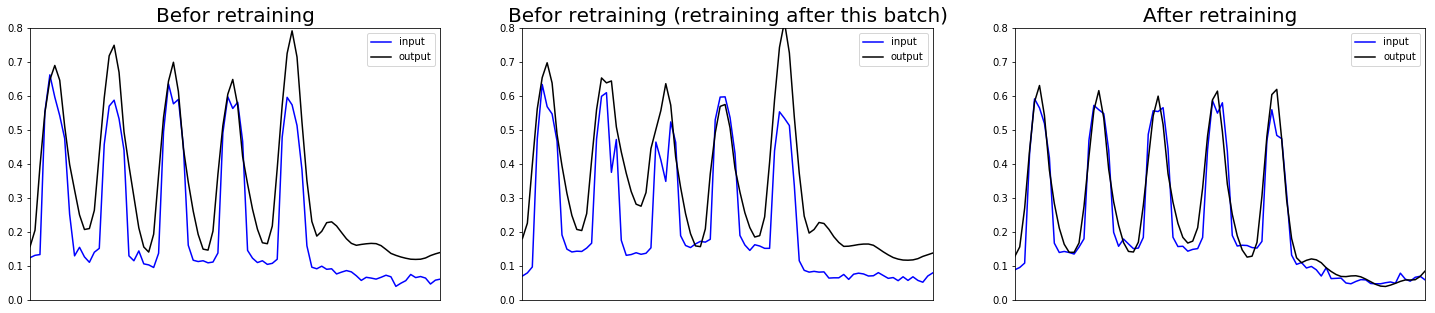
\includegraphics[width=15cm, height=4cm]{power_retraining}
\caption[Retraining effect on Power Demand dataset]{Retraining effect on Power Demand dataset}
\label{fig:power_retraining}
\end{figure}



\subsection{Comparasion: with and without retraining}
\label{sec: compare}

performance and reconstruction error\\
what data used for retraining


\subsection{Reaction of concept drift and distribution changes}
\label{sec:reaction}
observation of model perfermance around positions of concept drift and distribution changes 

\subsection{Running time analysis}
\label{sec:time}




